\section{DISCUSSION}
\subsection{Algorithm implementation}
As mentioned earlier in the above section, left wall following algorithm was implemented in the first robot in order to carry out the task of maze traversal. 
According to the aforementioned algorithm, the robot always tries to follow the left wall of the maze. Basically, the first step towards implementation of the algorithm was detection of the closest wall. \\
\begin{figure}[h]
\center
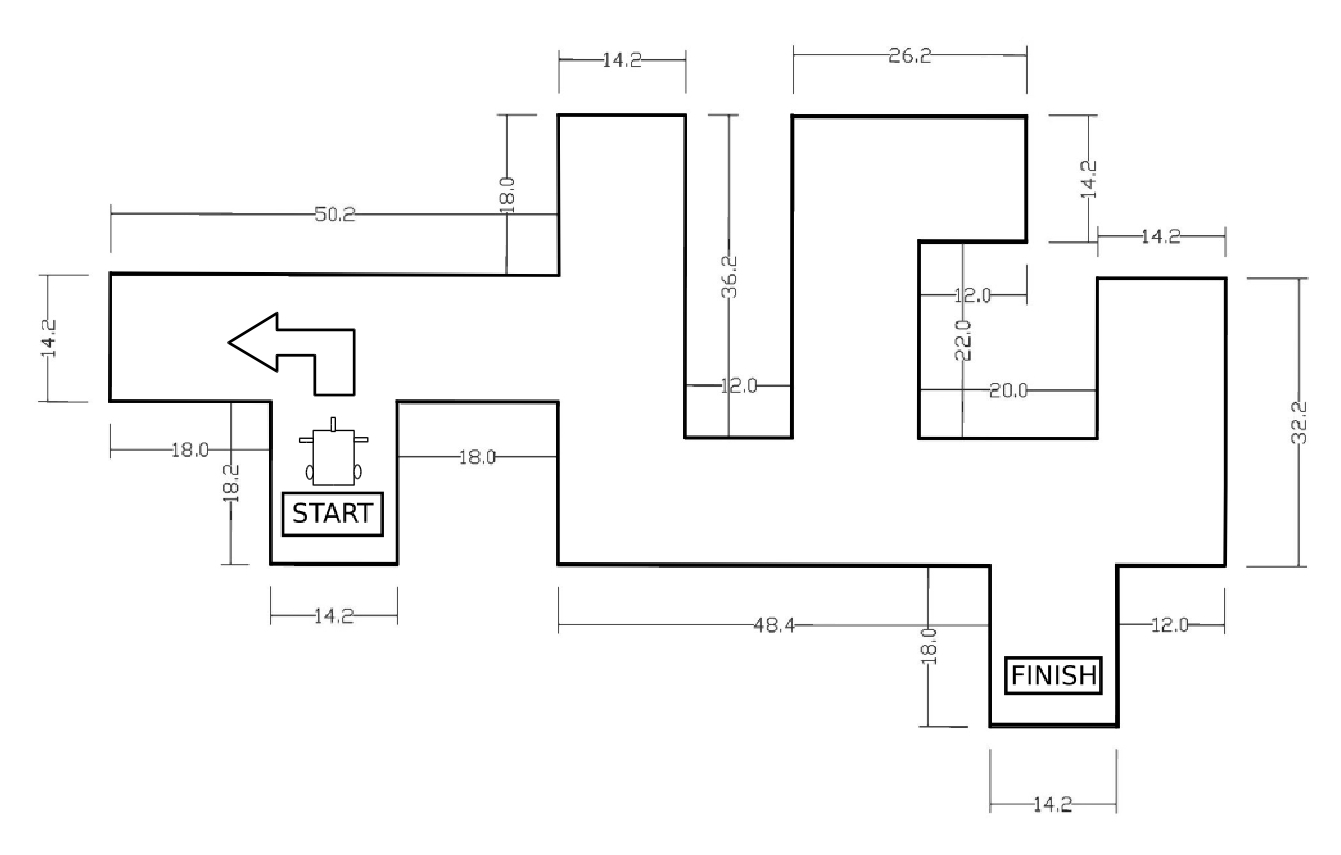
\includegraphics[scale=0.3]{part1_newnew.jpg}
\caption{Detection of the closest wall} 
\label{Firstplacementofthebot}
\end{figure}
\justify The robot followed the left wall until it encountered a junction where a decision had to be made. Based on this algorithm the robot turned left when there was an opening in the respective direction. In any condition that the left opening was blocked or there was a wall along the left side of the robot, the priority was transferred to the straight movement and it kept following the left wall until the next junction occurred. When both the left and front openings were blocked, the robot turned right provided there was an opening in that direction. Finally, when there was a blockade on all the three above mentioned sides viz. Left, straight and right, the robot decided to take a U-turn. 
Using this technique, the robot was able to traverse the maze up to the target point.\\
\begin{figure}[h]
\center
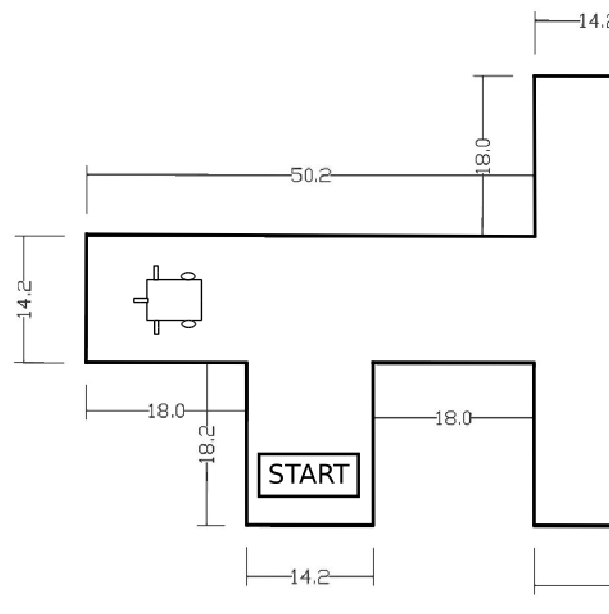
\includegraphics[scale=0.6]{part1_2new.jpg}
\caption{Robot following the left wall} 
\end{figure}
\justify From the above figure it can be seen that there is no any possible path for the robot's movement. Hence, it takes a U-turn as shown in the figure below.\\
\newpage
\begin{figure}[h]
\center
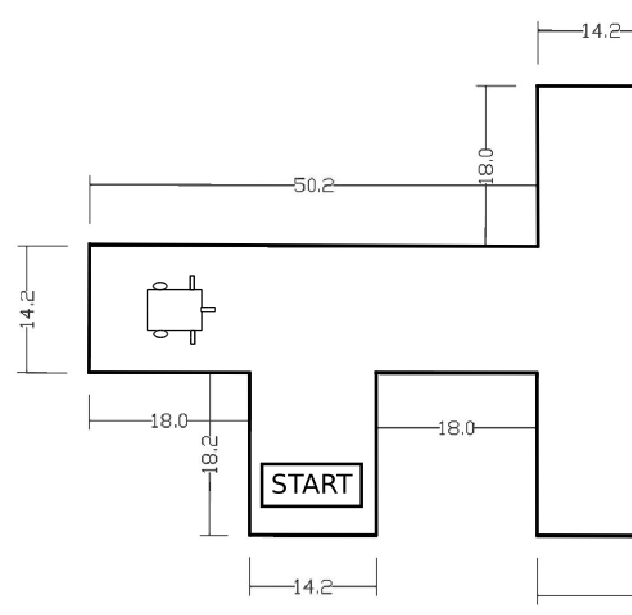
\includegraphics[scale=0.6]{part1_3new.jpg}
\caption{U-turn of the robot} 
\end{figure}
\subsection{Detection of the wall}
Detection of the wall was carried out through IR sensors. The IR sensor module FC-51 has a sensing range of up to 30cms. The left wall of the maze was detected by the IR sensor which was indicated by the LED present within the module. By adjusting the potentiometer of the sensor module, the IR was made to detect a wall at a distance of about 6-8 cms. Similarly, the sensors placed on the front and right side of the robot were able to successfully detect the respective walls.\\
The following image shows the working of the IR sensor module along the left wall.\\
\newpage
\begin{figure}[h]
       \begin{center}
       
       \begin{subfigure}[b]{0.5\textwidth}
                 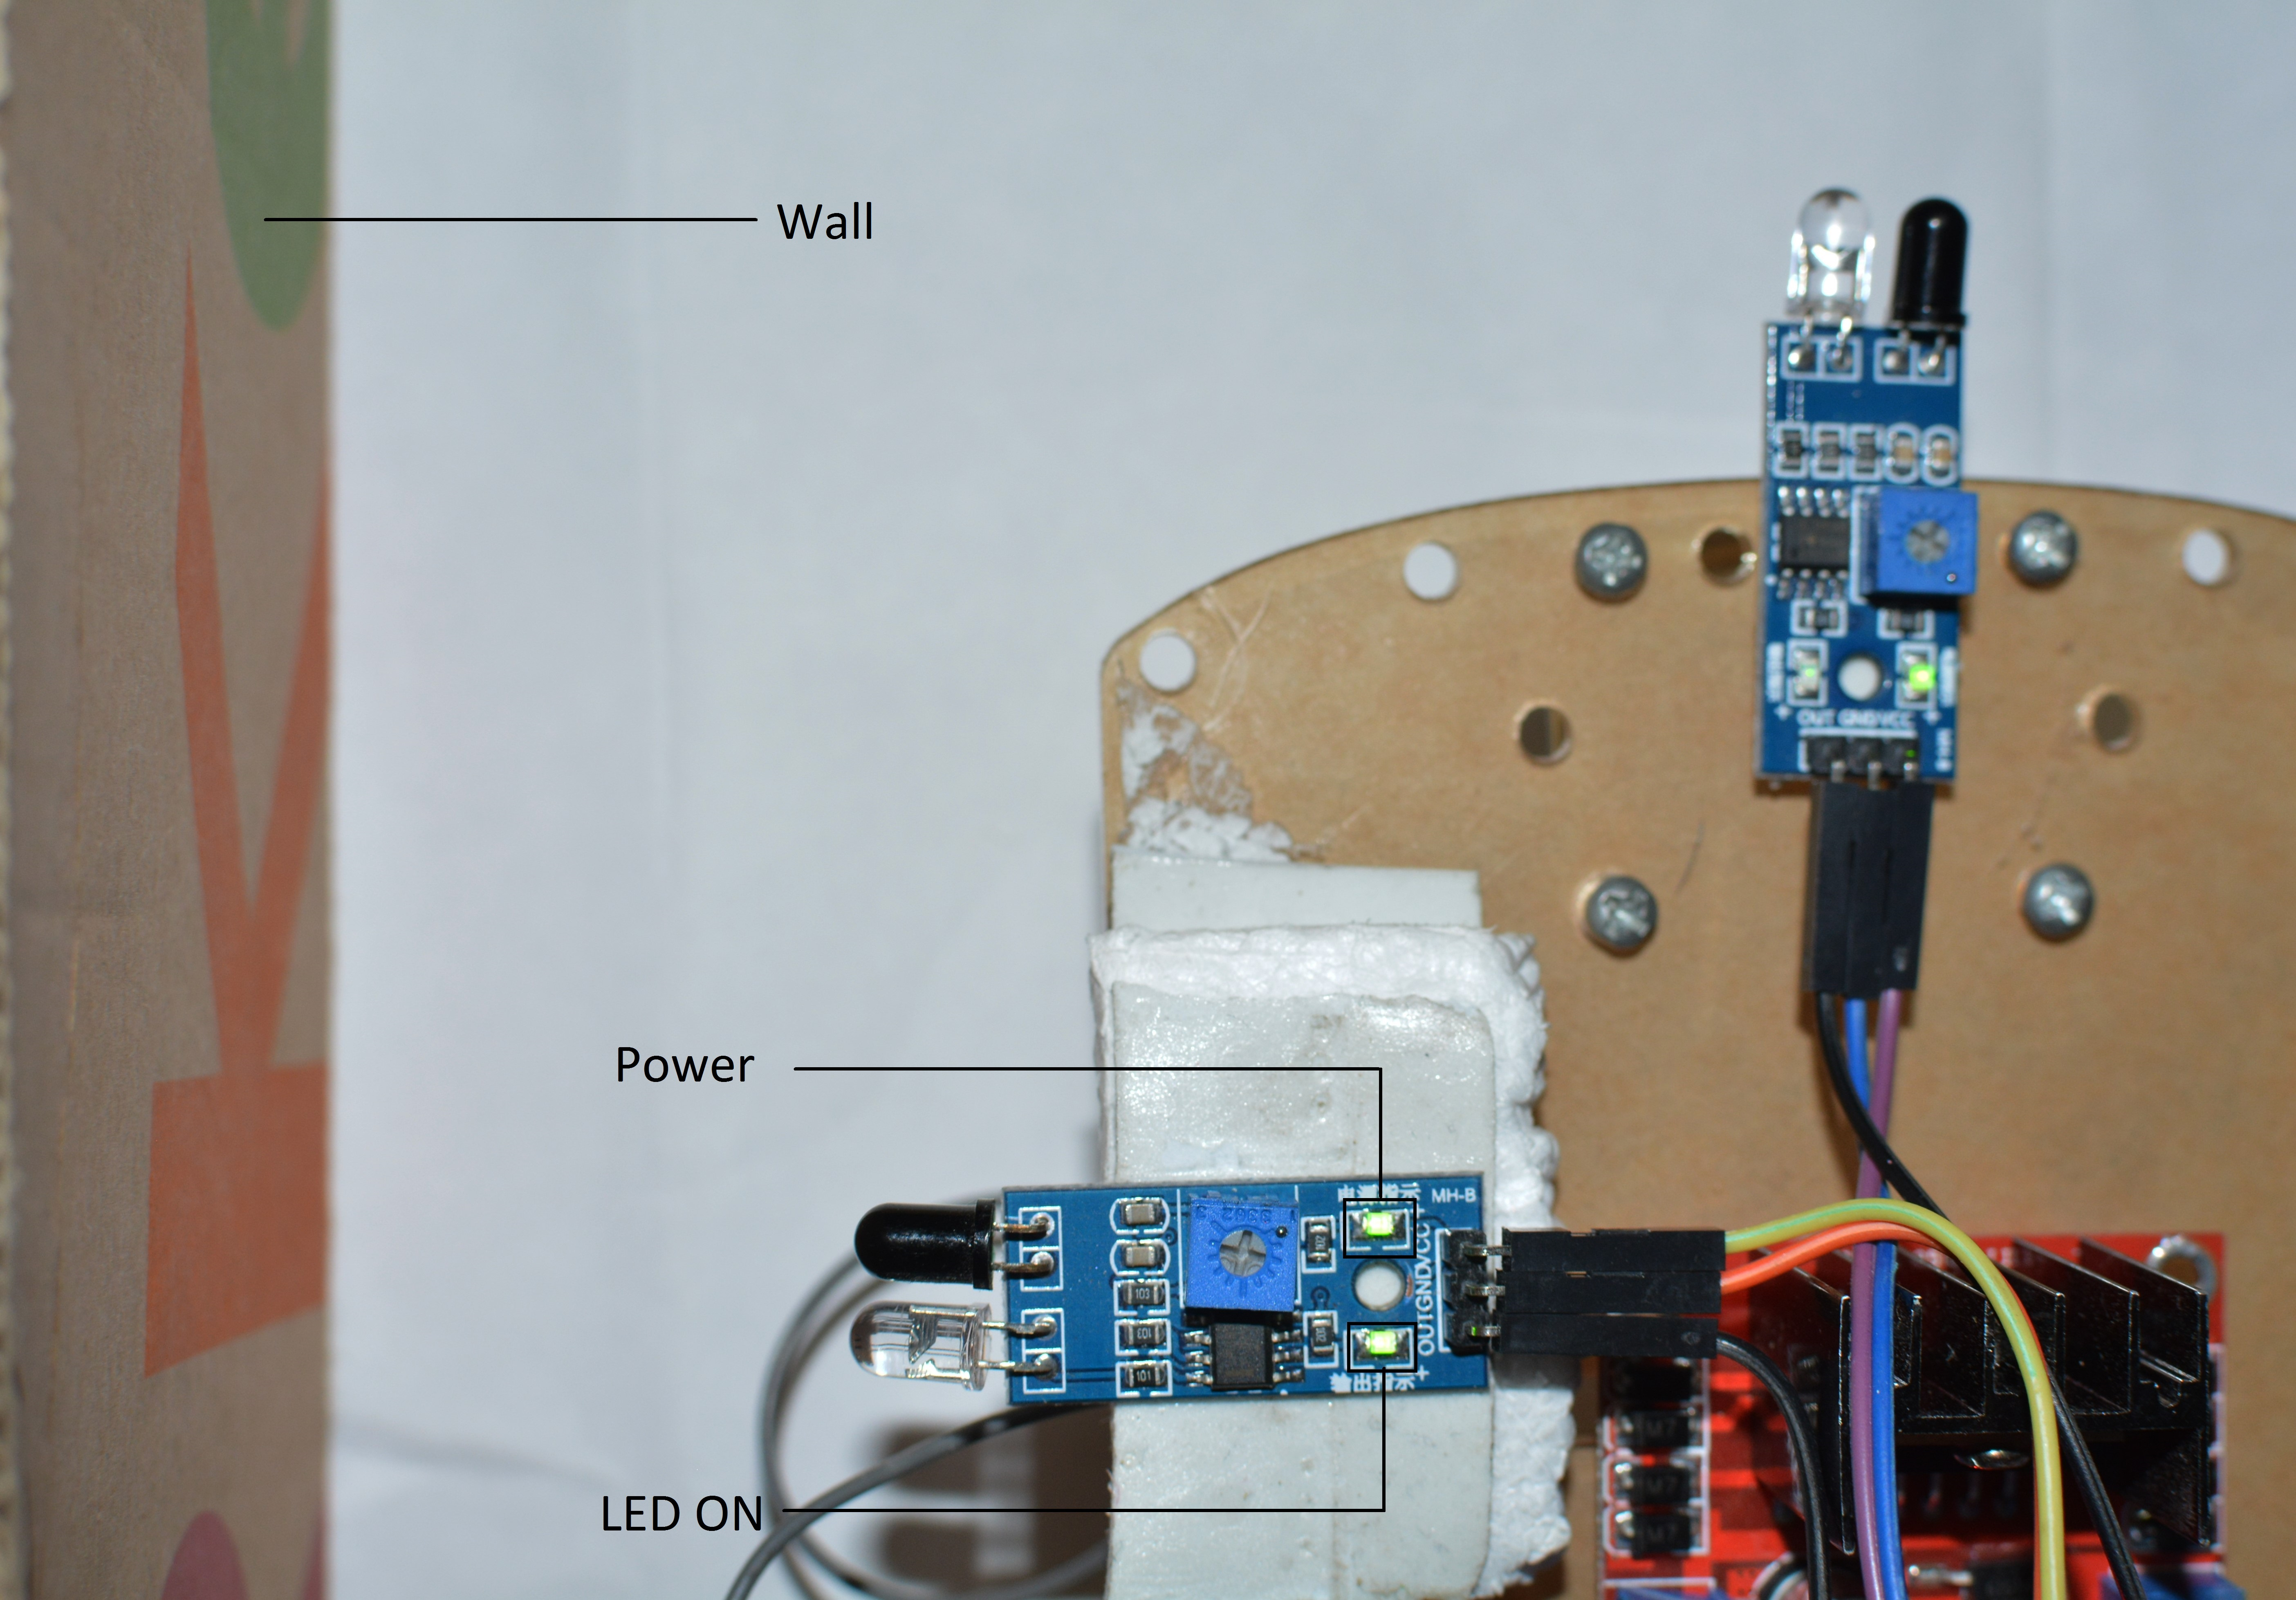
\includegraphics[scale=0.21]{part3_1_lb.jpg} 
                \caption{The detection of wall by the left sensor}
                
        \end{subfigure}
        \begin{subfigure}[b]{0.5\textwidth}
                  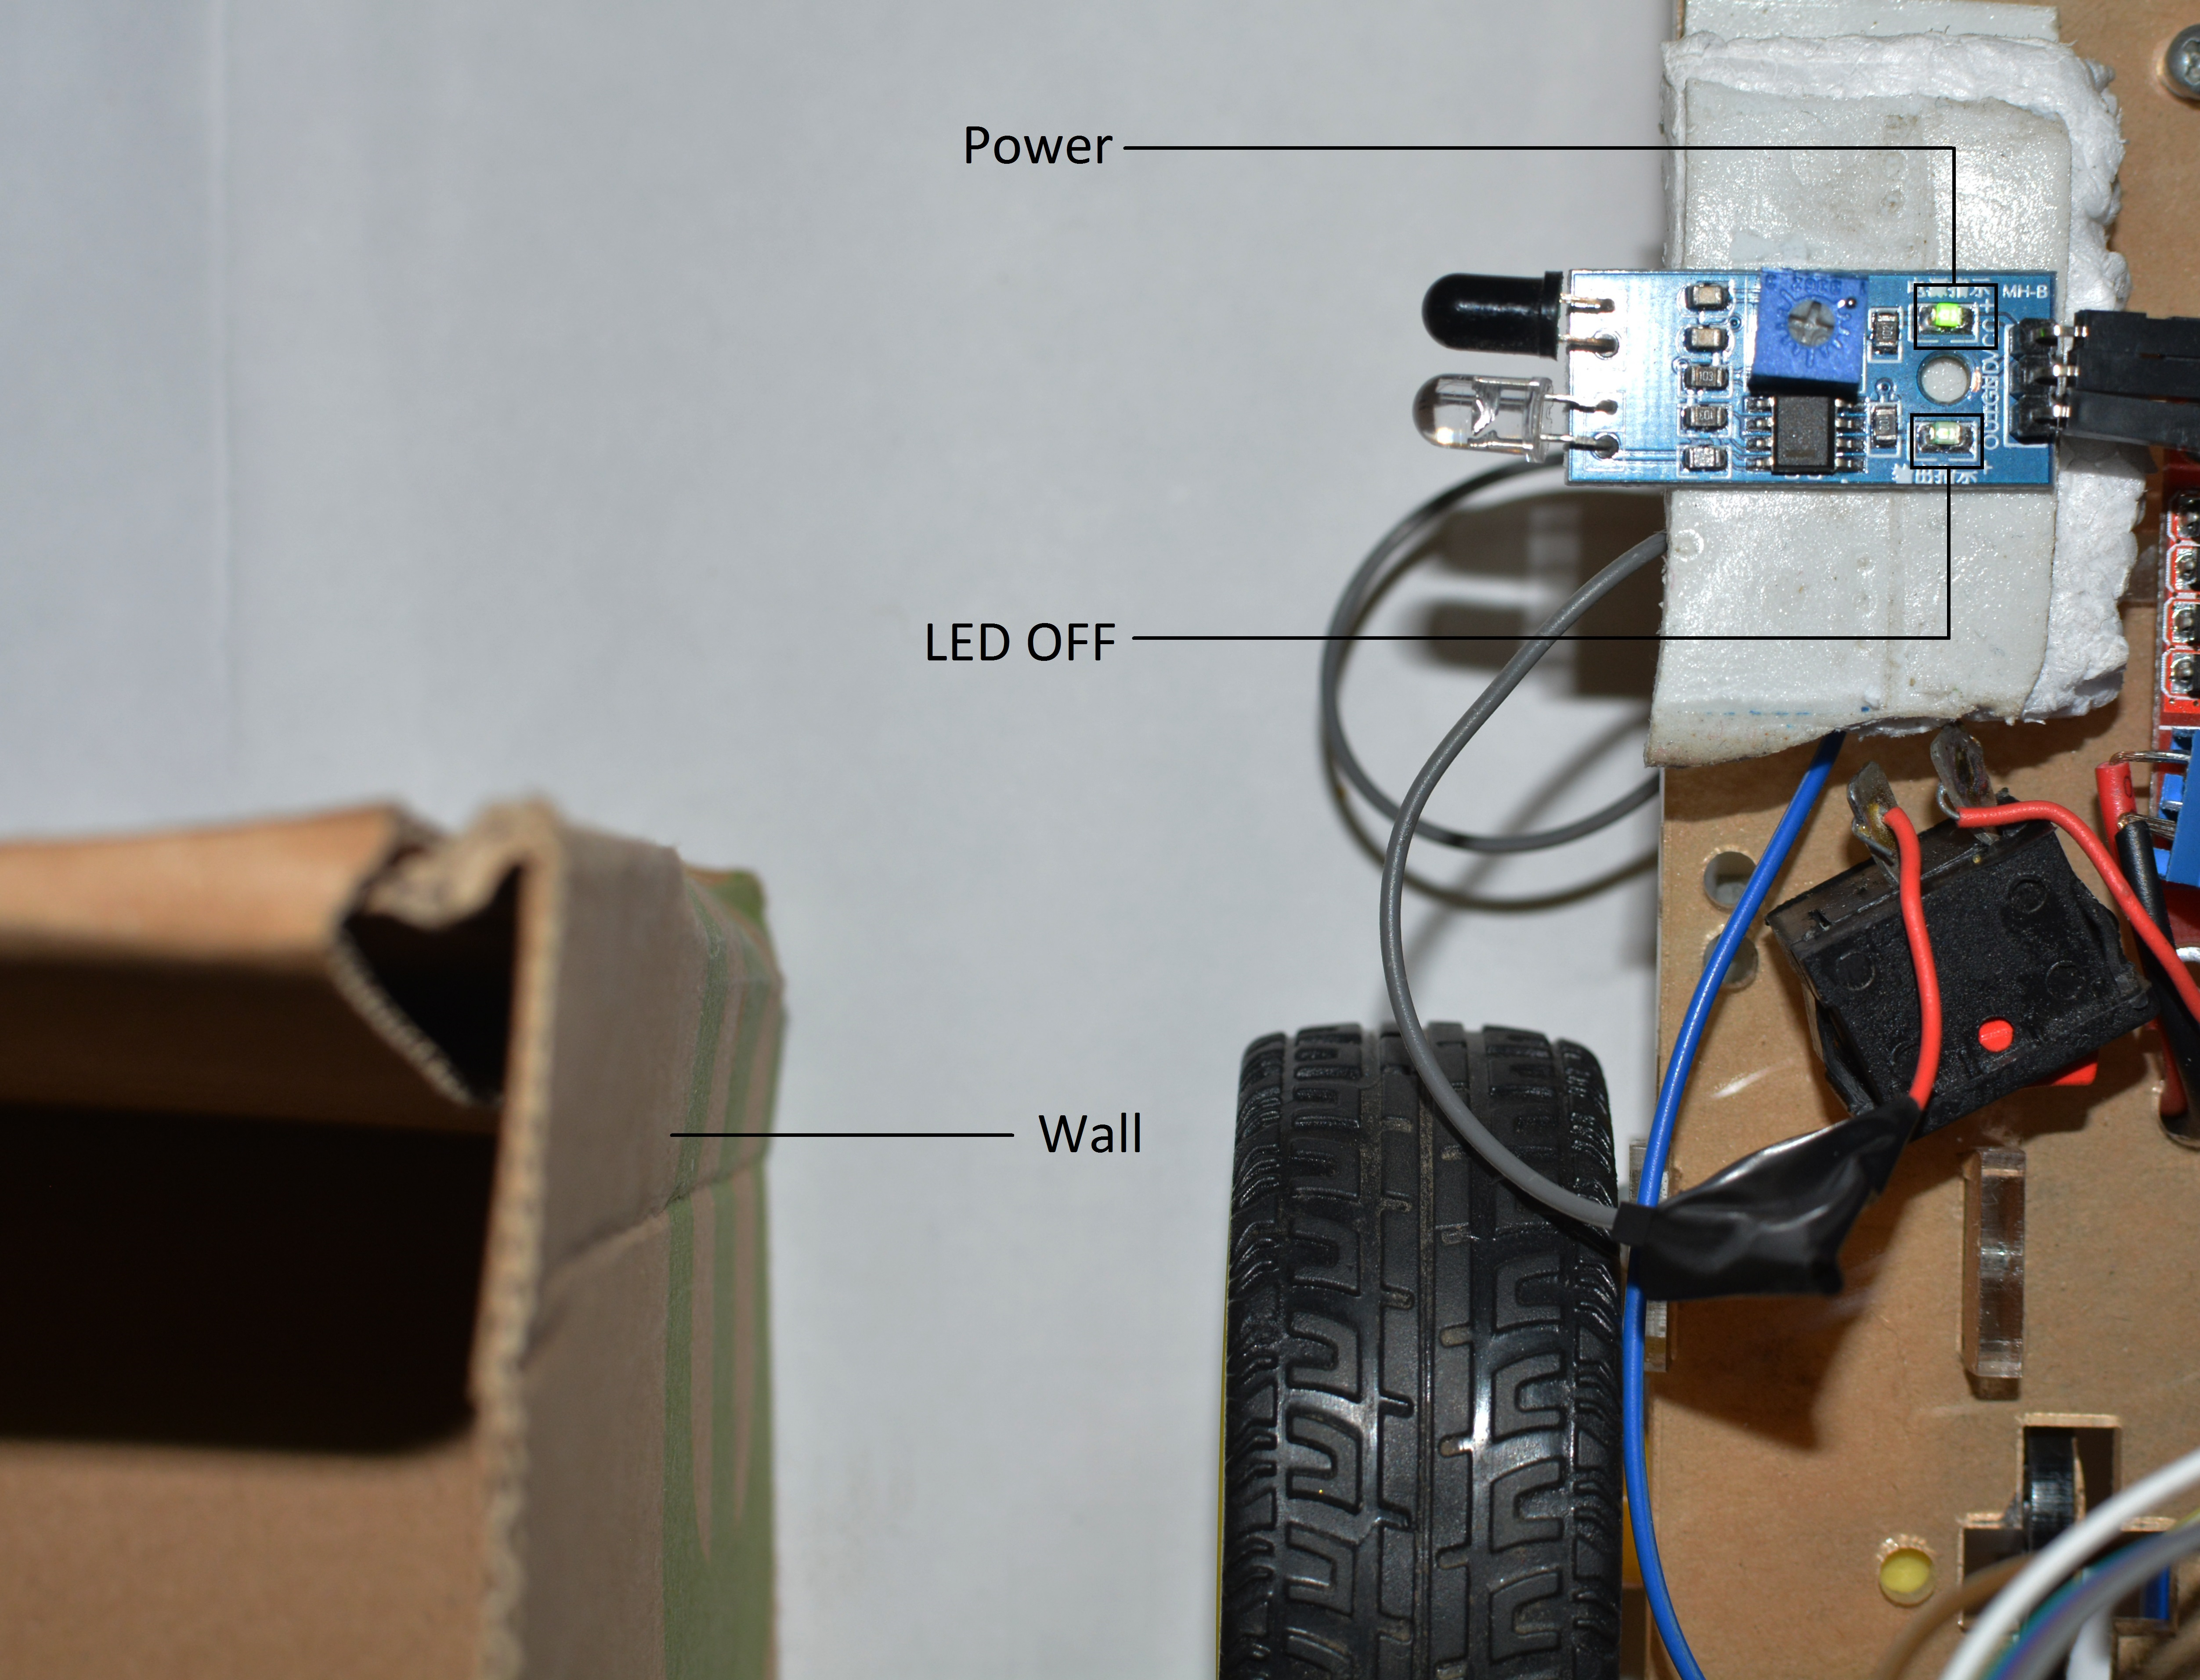
\includegraphics[scale=0.21]{part3_2_lb.jpg} 
                \caption{No detection of wall}
                \label{fig:gull2}
        \end{subfigure}%
        \caption{Implemenation of the IR sensor for detection of the left wall}
\end{center} 
\end{figure}
\justify Similarly, the following image shows the working of the IR at different distances from the front of the wall.\\
\newpage
\begin{figure}[h]
\begin{center}
        \begin{subfigure}[b]{0.5\textwidth}
                 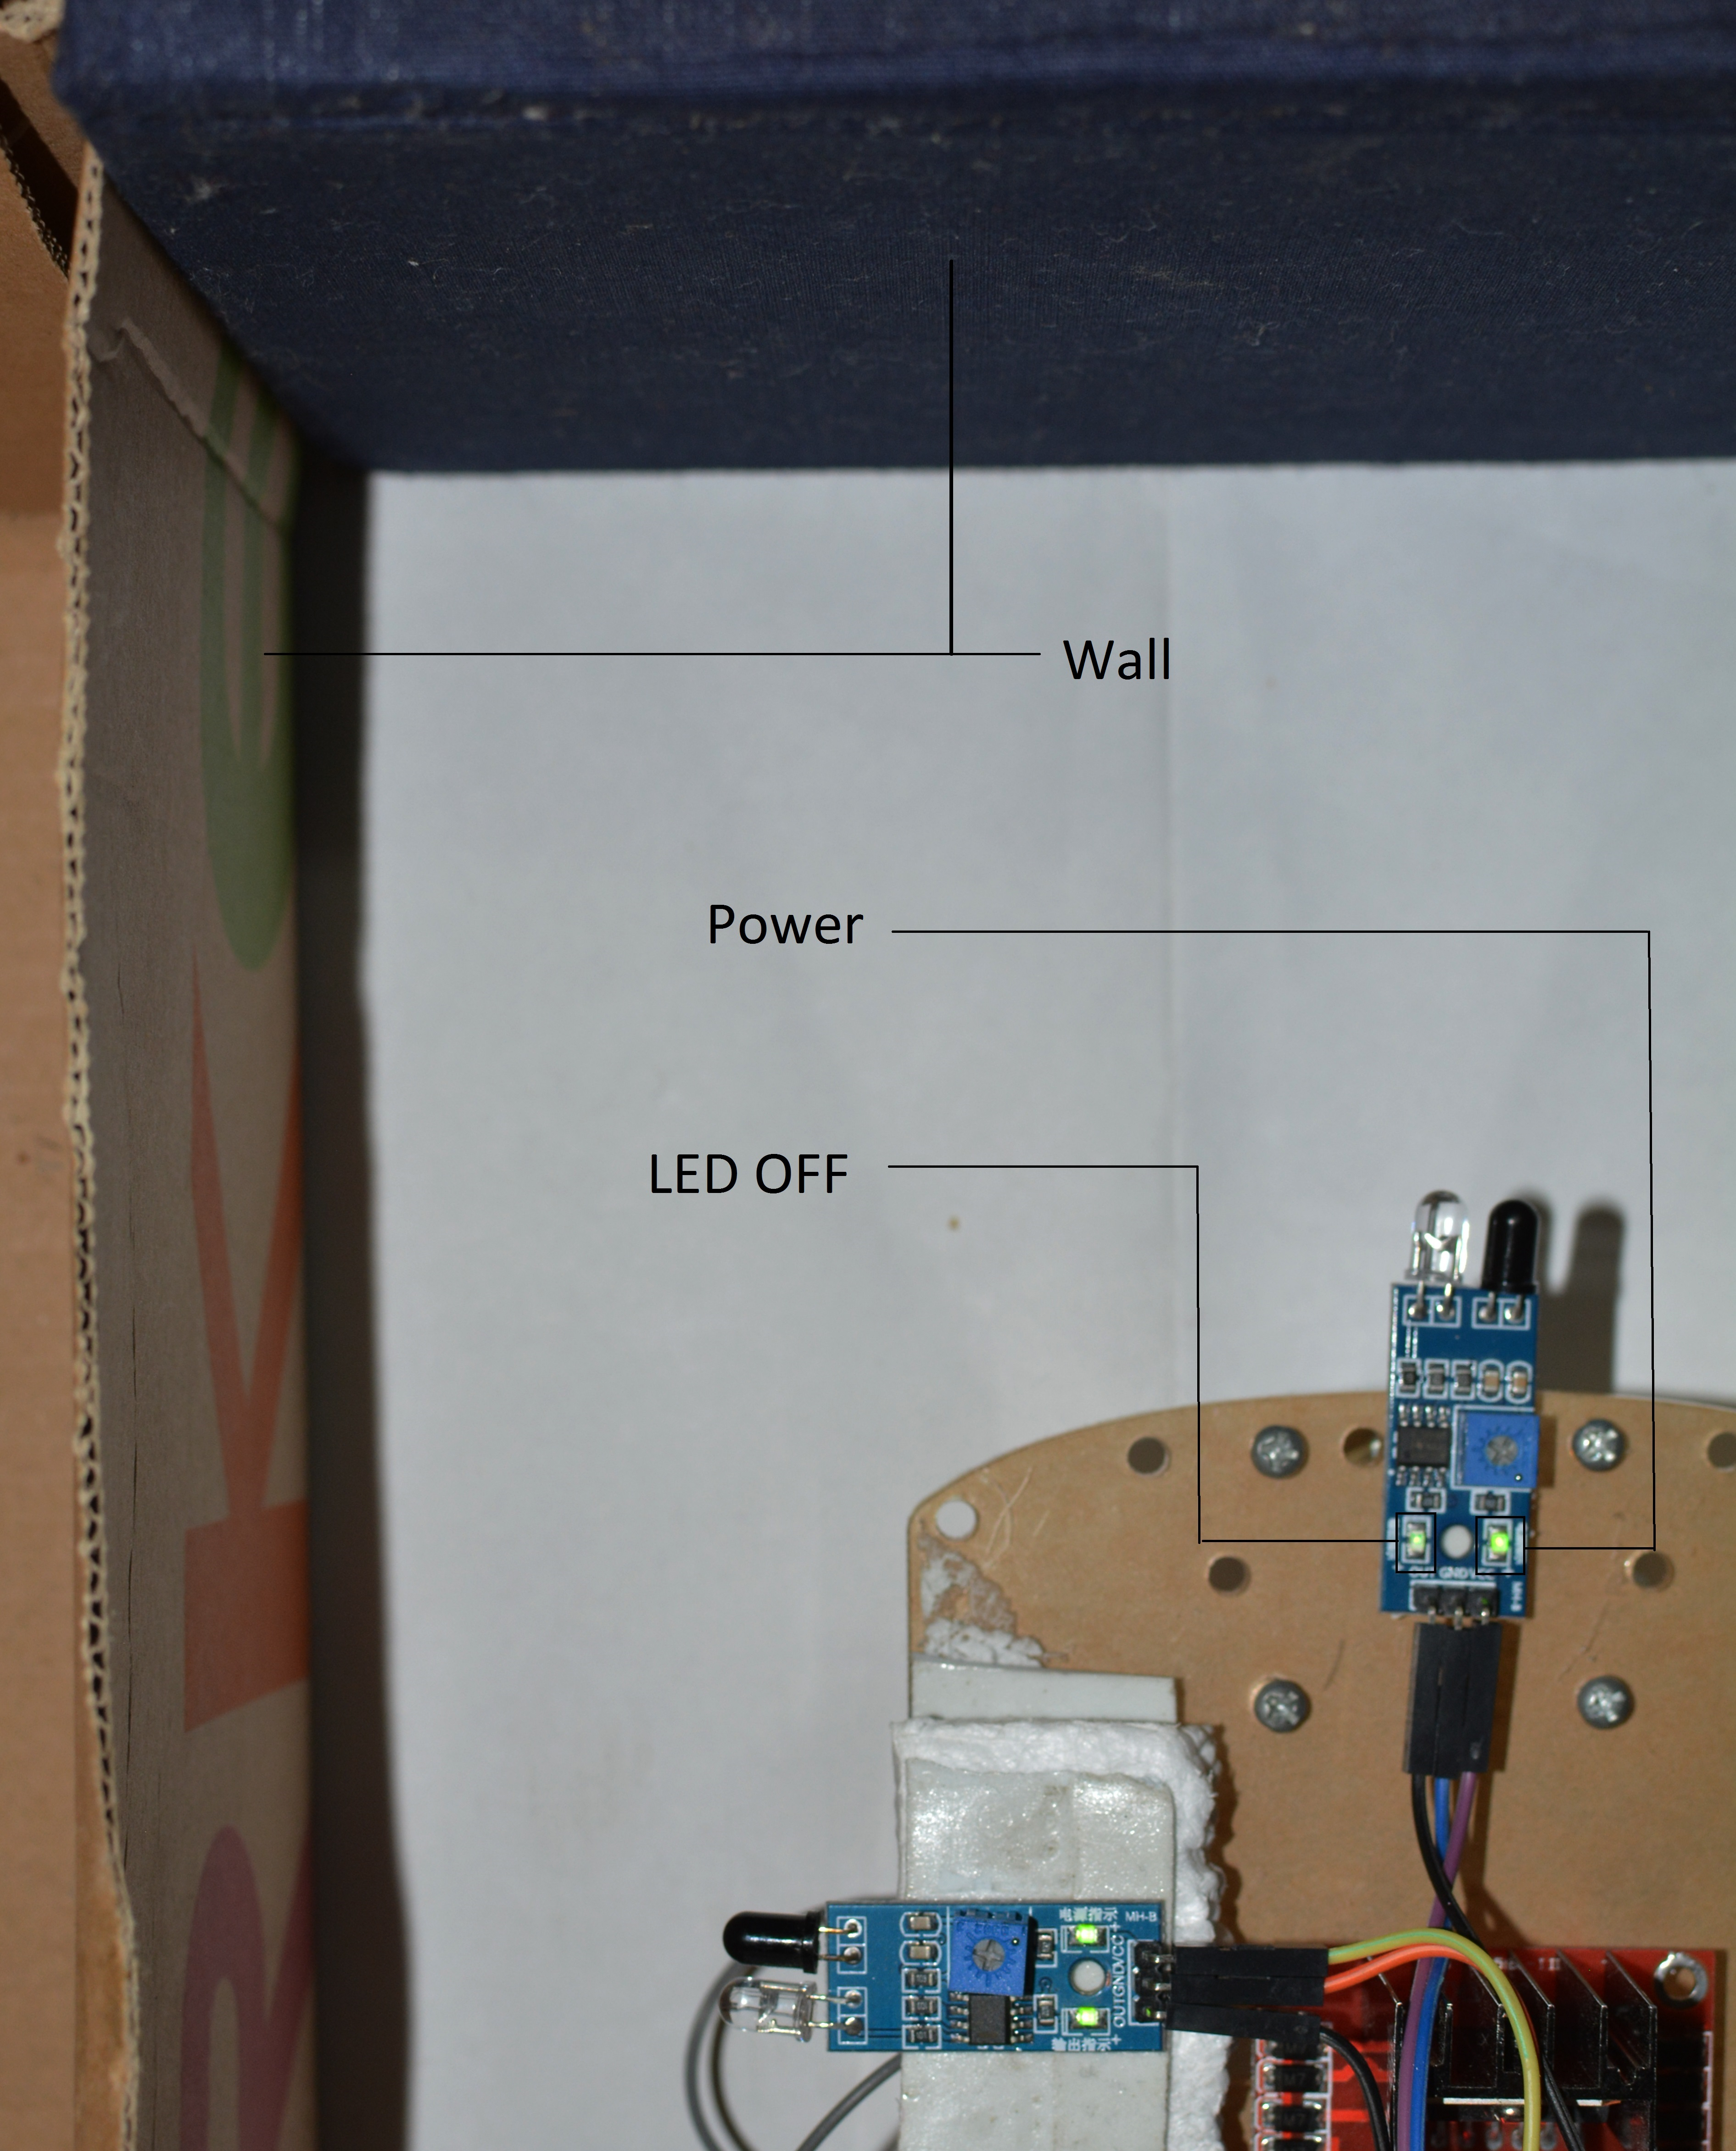
\includegraphics[scale=0.195]{part3_3_lb.jpg} 
                \caption{No detection of wall by the front sensor}
        \end{subfigure}
        \begin{subfigure}[b]{0.5\textwidth}
                  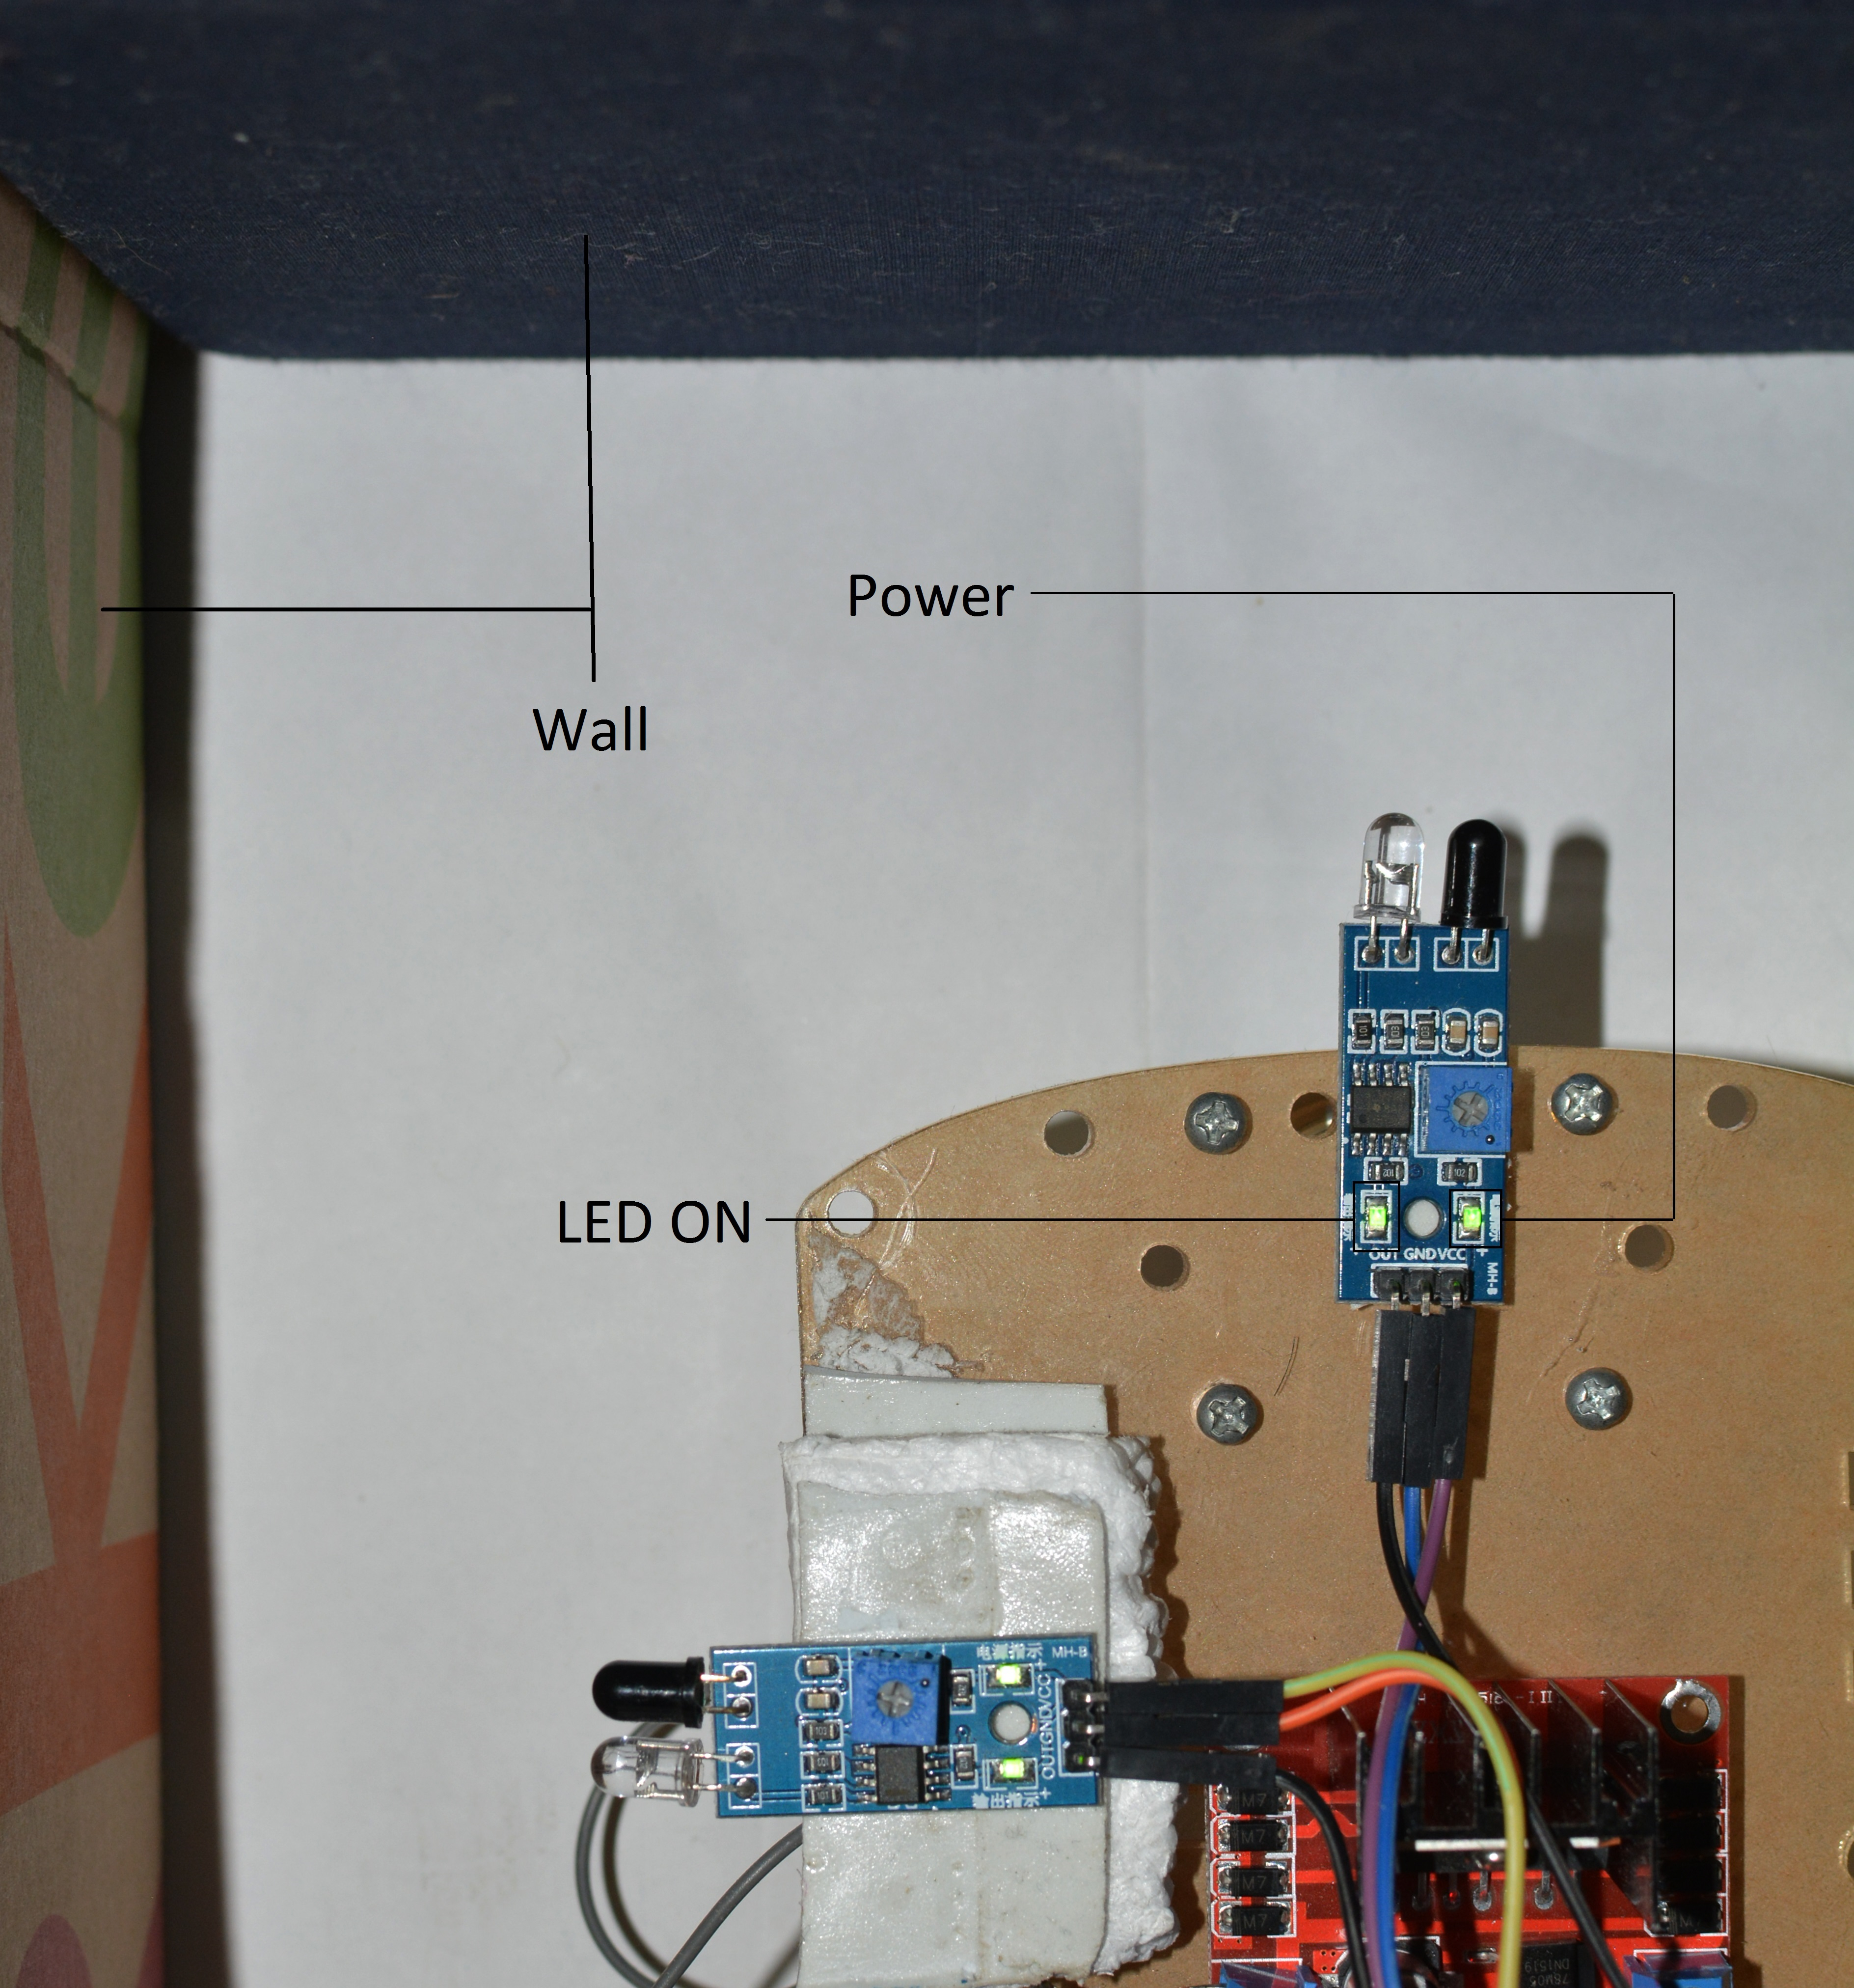
\includegraphics[scale=0.195]{part3_4_lb.jpg} 
                \caption{Detection of wall by the first sensor}
                
        \end{subfigure}
        \caption{Implemenation of the IR sensor for detection of the front wall at different distances}
\end{center} 
\end{figure}
\subsection{Path traversal by the second robot}
The second robot received the information/decision from the first robot and started traversing the maze. The junction in the maze was detected by a set of IR Sensors similar to that on the first robot.  Upon the arrival of the junction ,  the second robot took the desired decision that led the robot through the shortest path to the target.\\
Based on the above example, the result is shown below as: \\
Firstly, the second robot was placed at the initial position similar to as that of the first robot.
\begin{figure}[h]
\center
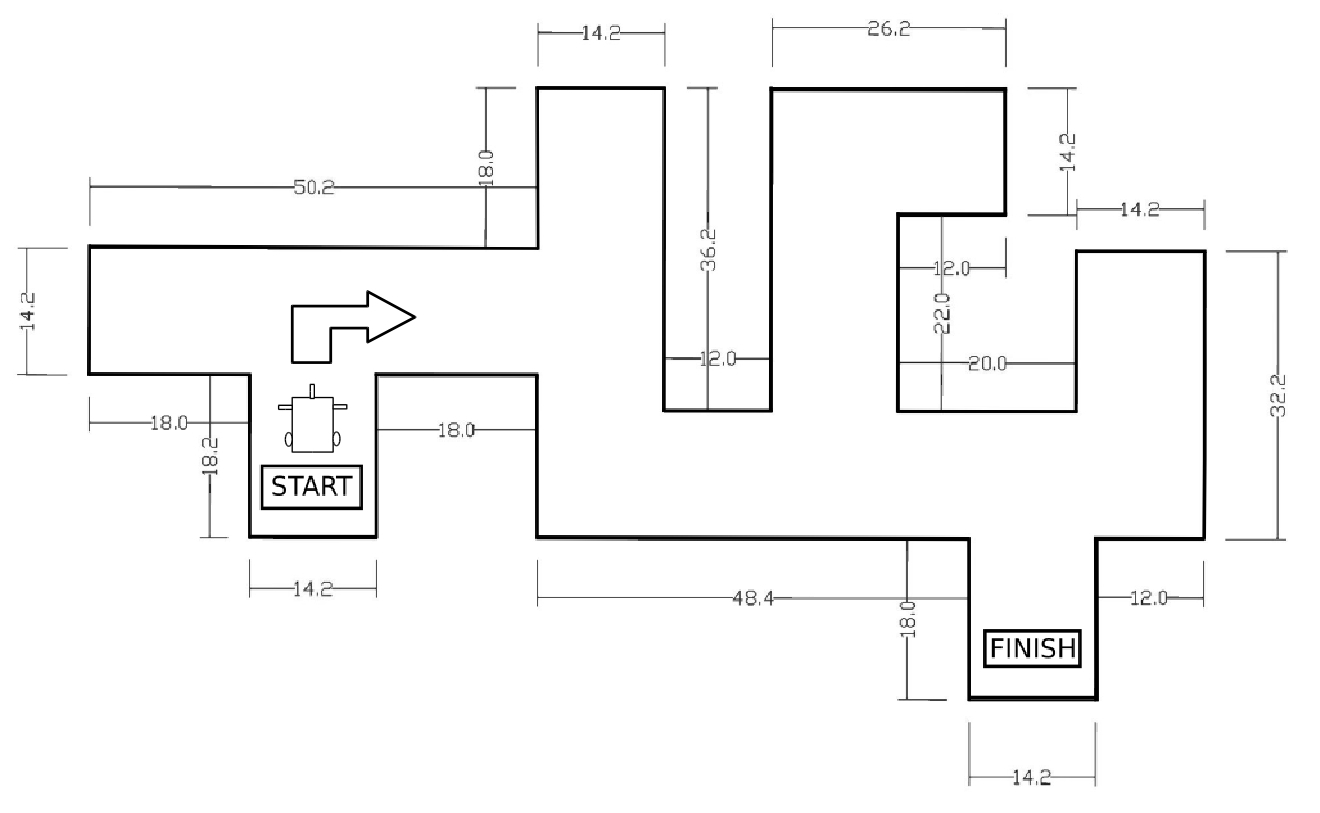
\includegraphics[scale=0.35]{part1_4new.jpg} 
\caption{Initial placement of the second robot similar to that as of the first robot}
\end{figure}
\justify Based on the left wall following algorithm, the first robot took the decision of following the left wall as shown earlier in the\ref{Firstplacementofthebot} Here, the second robot took the decision to go right based on the decoded packet sent by the first robot for reaching the target through the shortest path.\\
The robot movement continues through the shortest path throughout the maze all based upon the decoded packet.\\
\newpage
\begin{figure}[h]
\center
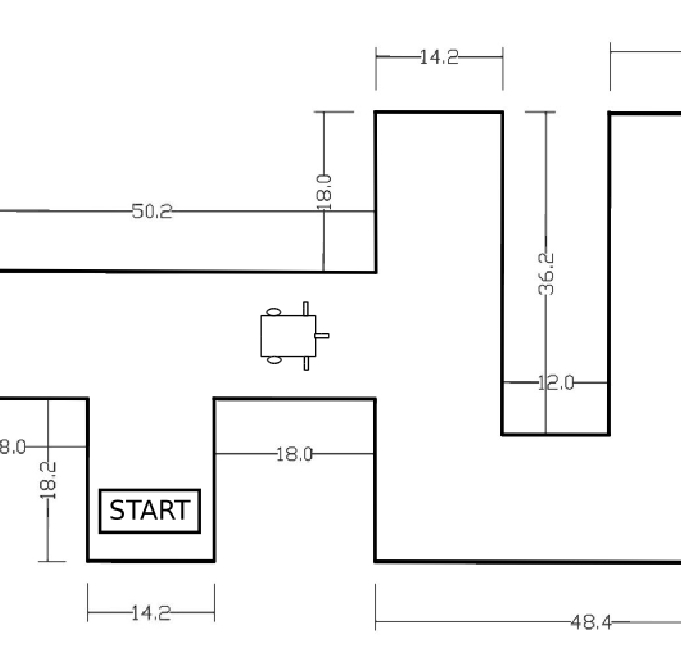
\includegraphics[scale=0.32]{part1_5new.jpg} 
\caption{Robot locomotion continues via the shortest possible path}
\end{figure}
\justify
On following the route provided by the first robot, the second robot ultimately reached the target.\\
\begin{figure}[h]
\center
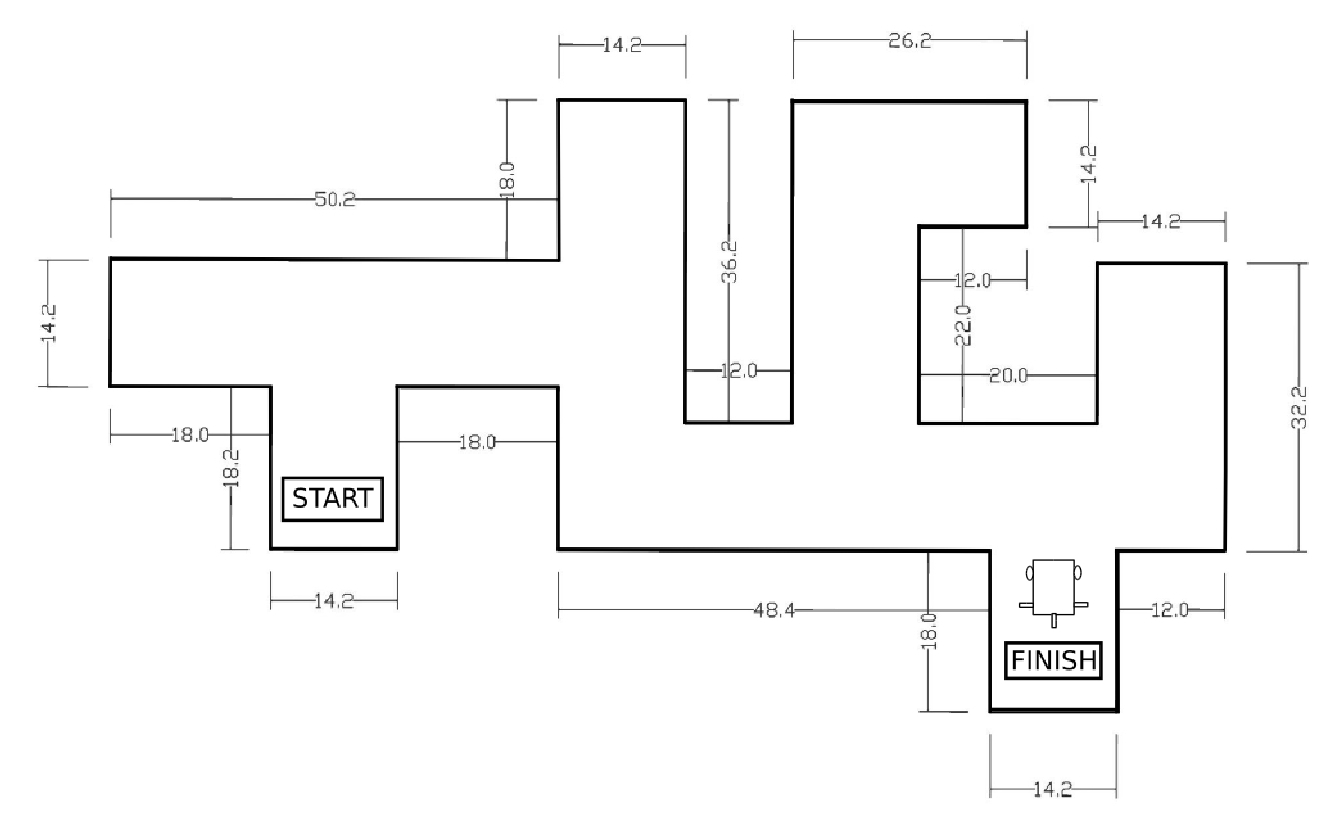
\includegraphics[scale=0.25]{part1_6new.jpg} 
\caption{Reaching of the target}
\end{figure}
\justify Thus, the route for the shortest path was obtained and implemented by the second robot successfully.
\subsection{Bluetooth Communication}
All the decisions required for solving the maze in the most efficient way were stored in a queue by the first robot which was then sent to the second robot via HC-05 Bluetooth module.\\
\begin{figure}[h]
\center
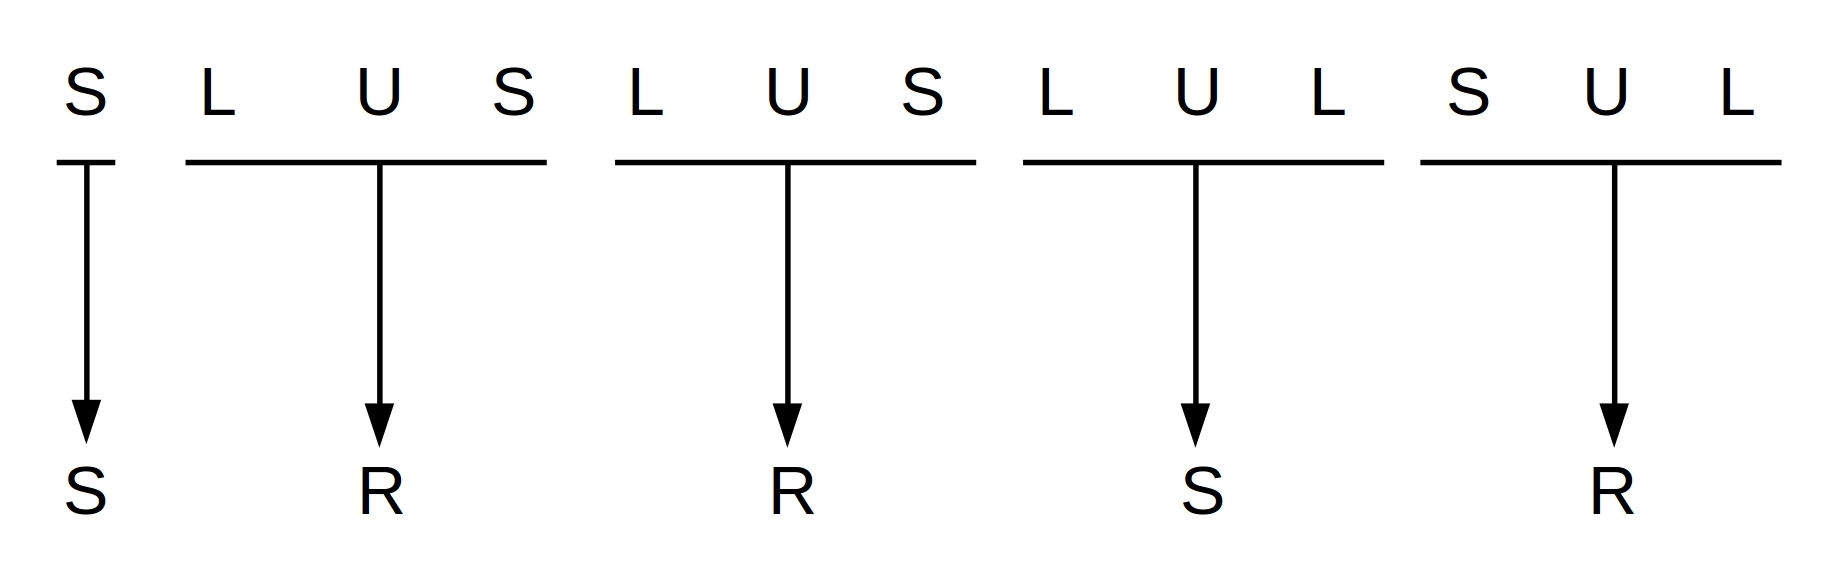
\includegraphics[scale=0.2]{decoding.jpg} 
\caption{Decoding Algorithm}
\end{figure}
\justify The figure above shows the decoding process of the junction decisions carried out by the first robot. This process is a \textit{"reduction process"} where the decisions taken by the first robot at respective junctions of the maze were re-examined and a more optimal result was extracted. The second robot traversed the maze according to this decoded packet of information and was able to reach the target through the shortest path possible.\\
The underlying algorithm behind this reduction process is to look for the occurrence of a U-turn (denoted by 'U'). For every occurrence of a U-turn, the robot adds the opposite decision that it took at the last junction  to the queue.\\
For example, if the robot reached a junction where it could go either left, (L) or drive straight (S)  it would turn left. But if it encountered a U-turn after taking the left turn, the opposite decision in the last junction i.e. straight, (S) would be added to the queue. \\
From the figure shown below, it can be seen that when the first robot encounters a U-turn for the first time, the decision not taken at the first junction is entered into the queue. So, the decisions L U S is replaced by R. \\
Similarly, the remaining occurrences of U-turns were decoded using this technique wherein L U L was converted to S and S U L to R. This way, the final junction decisions for the shortest path was extracted.\\
\begin{figure}[h]
\center
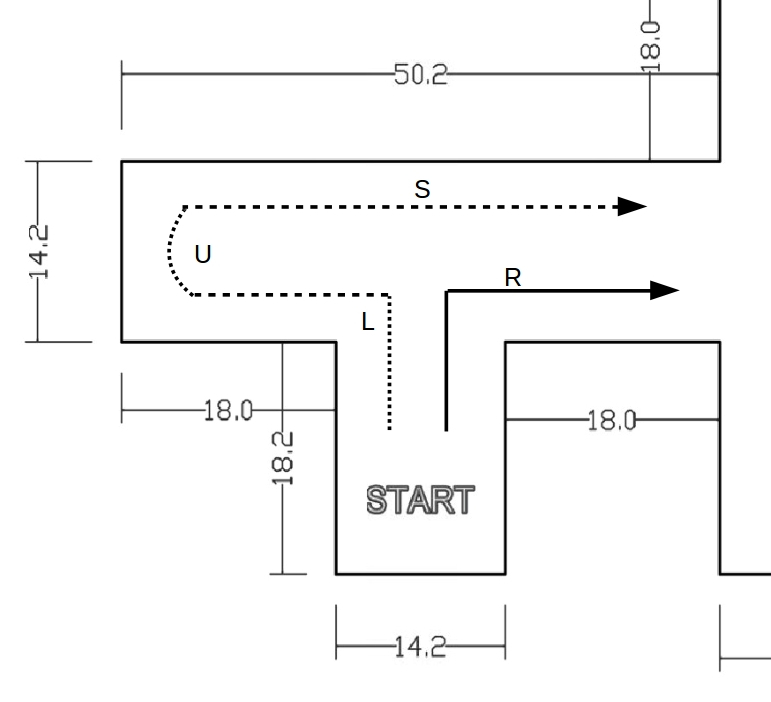
\includegraphics[scale=0.5]{deconding_1_final.jpg}
\caption{Implementation of \textit{reduction process}} 
\end{figure}
\subsection{Motor Synchronization}
Various problems and shortcomings were faced during the course of the progress of the project.However, most of them were overcome.\\
One of the first shortcoming was the synchronization of the two motors. Even though the two motors were identical in terms of specifications and manufacture, like all devices, they had inherent differences. As a result, the rate of rotation of the two motors were different and the bot failed to move in a perfectly straight line. This problem can be solved by using a closed control circuit, most probably using IR sensors to make a P-control system.
\subsection{Operation of Wheel}
Another shortcoming was the front wheel to be used in the robot. At first, a roller wheel was used  but with the rotation of the robot, the roller wheel rotated as well which changed the center of the weight of the robot thus hampering it's forward movement which resulted in non-uniform movement of the robot.\\
This shortcoming was overcomed with the use of the caster wheel. The use of caster wheel removed the problem of shifting of center of weight thus resulting in uniform motion.
\subsection{IR Sensors}
Another problem was the accuracy of the IR sensor module. Initially, various IR modules were tested to check the accuracy and distance up to which they operated. Most of them failed to correctly detect the maze walls at the proper distance. Hence, the modules used currently was the one selected to be used in the bot both in terms of accuracy and economy.\\
The IR transceiver pair was able to detect the obstacles i.e. the walls of the maze with the help of the reflection of the IR signals transmitted by the IR transmitting diode which were detected by the IR receivers. The potentiometer was used to adjust the resistance to one of the pins of the FC-51 which allowed us to adjust the sensing distance for the sensor.
\subsection{Power Source}
Selection and finding the best Li-Po battery of the required voltage and current specification was a daunting task and a 7.4v 1600mAh battery was selected as the most suitable choice. The Li-Po battery has a voltage rating of 7.4V. The output from this battery is provided to the L298N motor driver whose 5V output is used to drive the Arduino board. The 5V output from the Arduino Board is used to power the IR sensor module. \\
The output current capacity from the 5V output pin of the Arduino is ~500mA. According to the IR sensor module specification, the maximum current rating of each module is around 43mA when operating at 5V. Performing required calculations, four such sensors can be easily accommodated from the pin output of the board. \\
Furthermore, the connection of the Arduino to the motors was challenging in the sense that the output pins inherently had different clock frequencies and this resulted in the wheels rotating at different speeds. 
\subsection{PWM Generation}
The PWM signal was generation from microcontroller (ATMEGA 398). The H-Bridge was a interface between the microcontroller and DC motor. Using H-Bridge, the circuit was prevented from bursting. The battery would have to be inverted time and again if H-Bridge hadn't been used. The upper waveform is for Motor 1 and the lower one is for lower Motor 2 in all the figures shown in the result section. Motor should have stopped if same signal were passed to all the transistor of H-Bridge and same is the principal we have used for stopping the motor. The clockwise motion , anticlockwise motion and no motion was observed respectively. Between each clockwise and anticlockwise motion, delay of 3 seconds was observed.\\
\begin{figure}[h]
\center
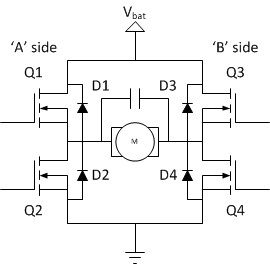
\includegraphics[scale=1]{hbridge.jpg} 
\caption{Diode configuration in H-Bridge}
\end{figure}
\justify The diodes (D1..D4) are called catch diodes and are usually of a Schottky type. Diode is basically a two-terminal electronic component that conducts primarily in one direction (asymmetric conductance). We need diodes for circuit to work. Without diodes, rest of the H-bridge gets killed at the moment motor turns off.\\
There are two types of elements that store energy: capacitors and inductors. Capacitors store charge because the energy can be stored statically.\\
Inductors cannot store energy statically. When circuit opens, they deliver that energy regardless if circuit is ready for it or not. Inductors are like railroad train which takes time to accelerate but it takes time to stop it. It does not stop instantly.  Inductors takes time for current flow through it to grow, but when the circuit is turned off, current does not stop instantly (even though you have open circuit). Inductor will keep on pushing that same current through whatever resistance that 'open circuit' is. Eventually voltage builds up until there is an insulation breakdown. If the insulator is air, we can see the spark. In case of H-Bridge, sparks are inside transistors.\\
So, we need diodes to divert running train to an alternate track so it has time to slow down, i.e, provide the path for the inductive "kick" that is generated when the motor is switched off in h-bridge circuit. Also, the diodes prevent back EMF when the motor is switched off.\\
For this, IN1 and IN4 were set high and IN2 and IN3 were set low. So, the current moved from IN1, through motor and then to IN4 of H-Bridge. As both EN1 and EN2 were given more than half the maximum value of PWM, both their waves are same. Even when the PWM value was changed, there was only the small change in waveform. The duty cycle here was 60 percent.  When the maximum value of PWM was given, the waves weren’t visible because the speed was too high. The current is flowing from the top left to buttom right in this case without flowing through IN2 and IN3. \\
Here, contrary to the case of clockwise direction, IN2 and IN3 were set high (1) while IN4 and IN5 were set low (0). The duty cycle here was 60 percent. The waves are narrower than that of the clockwise direction. In between clockwise and anticlockwise, delay of 100 ms was taken so that the motor may not have the chance of crashing on changing direction abruptly. The current is flowing from IN2, through the motor and to IN3, i.e, it is flowing from buttom left to top right.\\
In the case of leftward, pins IN1 and IN3 were set low while the remaining pins were high. The current thus moved from buttom left to buttom  right crossing the motor. IN 2 and IN 4 were given high, i.e, 1. The PWM values in this case were also the same as clockwise and anti- clockwise direction so, duty cycle was also the same, i.e, 60 percent. The wave of motor 1 is narrower like anticlockwise motion while in motor 2, the waves are wider like of clockwise motion.\\
For the rightward motion of the robot, IN1 and IN3 were set high, i.e, 1 and the remaining pins were low. The PWM value to ENA and ENB and also the duty cycle was same in this case too. The current here thus moved from top left to top right through the motor. If the direction had been reverse, the motor would have moved in left direction. Here, the wave of Motor 1 is wider like clockwise and Motor 2 has narrower wave like anticlockwise contrary to left sided motion.\\



